\chapter{Desarrollo}\label{ch:ch2label}

\section{Compilaci\'on}

Para la compilaci\'on del c\'odigo se utilizo un Makefile que se muestra a continuaci\'on:

\begin{tiny}

\begin{lstlisting}[numbers=left, tabsize=2, basicstyle=\fontsize{11}{13}\ttfamily, frame=single, caption={makefile}]
# makefile parameters
BIN_NAME    := tp
SRCDIR      := src
TESTDIR     := tests
BUILDDIR    := int
TARGETDIR   := target
SRCEXT      := c

# compiler parameters
CC          := gcc
CFLAGS      := -O3 -std=c99 -Wall -Wpedantic -Werror
LIB         :=
INC         := /usr/local/include
DEFINES     :=


#-----------------------------------------------
# DO NOT EDIT BELOW THIS LINE
#-----------------------------------------------

# binaries file names
# each binary source code is expected to be in $(SRCDIR)/<binary>
TARGET := $(TARGETDIR)/$(BIN_NAME)

# sets the src directory in the VPATH
VPATH := $(SRCDIR)

# sets the build directory based on the binary
BUILDDIR := $(BUILDDIR)

# source files
SRCS := $(shell find $(SRCDIR) -type f -name *.$(SRCEXT))

# object files
OBJS := $(patsubst %,$(BUILDDIR)/$(BIN_NAME)/%,$(SRCS:.$(SRCEXT)=.o))

# includes the flag to generate the dependency files when compiling
CFLAGS += -MD


# special definitions used for the unit tests
ifeq ($(MAKECMDGOALS),tests)
    # adds an extra include so the tests can include the sources
	INC += src

	# sets the special define for tests
	DEFINES := __TESTS__ $(DEFINES)

	# includes the tests directory in the VPATH
	VPATH := $(TESTDIR) $(VPATH)

	# test sources
	TEST_SRCS := $(shell find $(TESTDIR) -type f -name *.$(SRCEXT))

	# test objects
	OBJS := $(patsubst $(BUILDDIR)/$(BIN_NAME)/%,$(BUILDDIR)/tests/%,$(OBJS))
	OBJS := $(patsubst %,$(BUILDDIR)/tests/%,$(TEST_SRCS:.$(SRCEXT)=.o)) $(OBJS)
endif

# adds the include prefix to the include directories
INC := $(addprefix -I,$(INC))

# adds the lib prefix to the libraries
LIB := $(addprefix -l,$(LIB))

# adds the define prefix to the defines
DEFINES := $(addprefix -D,$(DEFINES))


# builds the binary
$(TARGET): $(OBJS) | dirs
	@$(CC) $(CFLAGS) $(INC) $(DEFINES) $^ $(LIB) -o $@
	@echo "LD $@"

# compiles the tests
tests: $(TARGET) | dirs
	python tests/run.py $(TARGET)

# shows usage
help:
	@echo "Para compilar el binario:"
	@echo
	@echo "\t\033[1;92m$$ make\033[0m"
	@echo
	@echo "Para compilar y ejecutar las pruebas (require python 2.7+ instalado):"
	@echo
	@echo "\t\033[1;92m$$ make tests\033[0m"
	@echo
	@echo "Los binarios compilados se encuentran en \033[1;92m$(TARGETDIR)\033[0m."
	@echo

# clean objects and binaries
clean:
	@$(RM) -rf $(BUILDDIR) $(TARGETDIR)

# creates the directories
dirs:
	@mkdir -p $(TARGETDIR)
	@mkdir -p $(BUILDDIR)

# rule to build object files
$(BUILDDIR)/$(BIN_NAME)/%.o $(BUILDDIR)/tests/%.o: %.$(SRCEXT)
	@mkdir -p $(basename $@)
	@echo "CC $<"
	@$(CC) $(CFLAGS) $(INC) $(DEFINES) $(LIB) -c -o $@ $<


.PHONY: clean dirs tests

# includes generated dependency files
-include $(OBJS:.o=.d)
\end{lstlisting}

\end{tiny}

Para la compilaci\'on del c\'odigo basta con ejecutar el Makefile:

\begin{lstlisting}
$ make 
\end{lstlisting}

\section{Corridas de prueba}

A la hora de ejecutar las pruebas, basta usar el mismo Makefile pero ahora con lo opci'on \textbf{tests}:

\begin{lstlisting}
$ make tests
\end{lstlisting}

\subsection{Resultados}

Se utilizaron los 4 archivos de palabras provistos, con los siguientes tama\~nos (en MiB):

\begin{center}

 \begin{tabular}{|c | c|} 
 \hline
  & Size  \\ 
 \hline\hline
Alice & 0.17 \\
\hline
Beowul/f & 0.21 \\
\hline
Cyclopedia & 0.63  \\
\hline
El quijote & 2.1 \\
 \hline
\end{tabular}\\
\end{center}

En la siguiente tabla se muestran los timpos (en segundos) que se tard\'o en ejecutar el programa con cada entrada:

\begin{center}
 \begin{tabular}{|c | c c c c|} 
 \hline
  & Count Bytes & Count Chars & Count words & Count lines \\
 \hline\hline
Alice  & 0.082 & 0.102 & 0.113 & 0.066 \\
\hline
Beowul/f & 0.113 & 0.133 & 0.125 & 0.102 \\
\hline
Cyclopedia  & 0.25 & 0.348 & 0.301 & 0.234 \\
\hline
El quijote & 0.816 & 1.133 & 1 & 0.75 \\
 \hline
\end{tabular}

\end{center}

En base a estos resultados se pueden realizar gr\'aficos para evidenciar la tendencia como se muestran en \ref{some example}

\begin{figure}
\subfloat[]{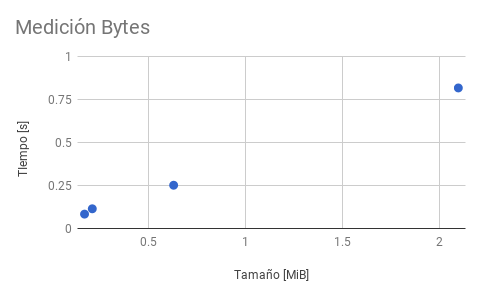
\includegraphics[width = 3in]{figures/chart(0).png}} 
\subfloat[]{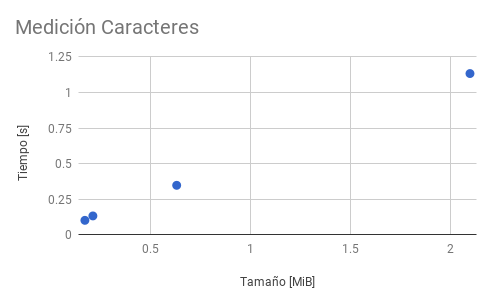
\includegraphics[width = 3in]{figures/chart(1).png}}\\
\subfloat[]{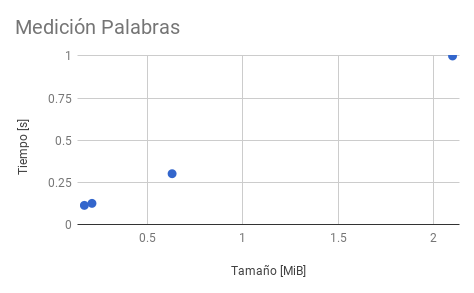
\includegraphics[width = 3in]{figures/chart(2).png}}
\subfloat[]{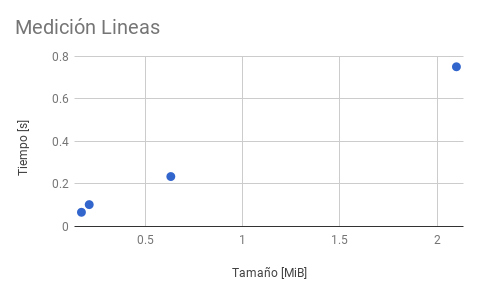
\includegraphics[width = 3in]{figures/chart(3).png}} 
\caption{Gr\'aficos de resultados obtenidos para cada valor de entrada}
\label{some example}
\end{figure}

\subsection{Resultados utilizando MIPS}

Utilizando la m\'aquina virtual, se obtuvieron las mediciones de tiempo utilizando la utilidad \textbf{time}. Los resultados se muestran en la tabla \ref{mipsresult}.


\begin{table}[]
\centering
\caption{My caption}
\label{my-label}
\begin{tabular}{l|l|l|l|l|l|}
\cline{2-6}
                                                  & Count Type & count   & real     & user     & sys      \\ \hline \hline
\multicolumn{1}{|c|}{\multirow{4}{*}{Alice}}      & Bytes      & 177428  & 0m0.082s & 0m0.066s & 0m0.016s \\ \cline{2-6} 
\multicolumn{1}{|c|}{}                            & Chars      & 177412  & 0m0.102  & 0m0.098s & 0m0.004s \\ \cline{2-6} 
\multicolumn{1}{|c|}{}                            & Words      & 30357   & 0m0.113s & 0m0.066s & 0m0.035s \\ \cline{2-6} 
\multicolumn{1}{|c|}{}                            & Lines      & 4046    & 0m0.066s & 0m0.066s & 0m0.000s \\ \hline
\multicolumn{1}{|c|}{\multirow{4}{*}{Beowulf}}    & Bytes      & 224839  & 0m0.113s & 0m0.086s & 0m0.027s \\ \cline{2-6} 
\multicolumn{1}{|c|}{}                            & Chars      & 224806  & 0m0.133s & 0m0.113s & 0m0.020s \\ \cline{2-6} 
\multicolumn{1}{|c|}{}                            & Words      & 37048   & 0m0.125s & 0m0.121s & 0m0.004s \\ \cline{2-6} 
\multicolumn{1}{|c|}{}                            & Lines      & 4562    & 0m0.102s & 0m0.082s & 0m0.020s \\ \hline
\multicolumn{1}{|l|}{\multirow{4}{*}{Cyclopedia}} & Bytes      & 658543  & 0m0.250s & 0m0.242s & 0m0.008s \\ \cline{2-6} 
\multicolumn{1}{|l|}{}                            & Chars      & 658543  & 0m0.348s & 0m0.332s & 0m0.016s \\ \cline{2-6} 
\multicolumn{1}{|l|}{}                            & Words      & 105582  & 0m0.301s & 0m0.293s & 0m0.008s \\ \cline{2-6} 
\multicolumn{1}{|l|}{}                            & Lines      & 17926   & 0m0.234s & 0m0.223s & 0m0.012s \\ \hline
\multicolumn{1}{|l|}{\multirow{4}{*}{El Quijote}} & Bytes      & 2198907 & 0m0.816s & 0m0.789s & 0m0.027s \\ \cline{2-6} 
\multicolumn{1}{|l|}{}                            & Chars      & 2155340 & 0m1.133s & 0m1.094s & 0m0.020s \\ \cline{2-6} 
\multicolumn{1}{|l|}{}                            & Words      & 389470  & 0m1.000s & 0m0.980s & 0m0.020s \\ \cline{2-6} 
\multicolumn{1}{|l|}{}                            & Lines      & 37862   & 0m0.750s & 0m0.734s & 0m0.016s \\ \hline
\end{tabular}
\end{table}

\section{C\'odigo Fuente}


A contiunaci\'on se muestra el c\'odigo fuente:

\begin{tiny}
\begin{lstlisting}[numbers=left, tabsize=2, basicstyle=\fontsize{11}{13}\ttfamily, frame=single, caption={c\'odigo fuente del programa}]
#include <ctype.h>
#include <getopt.h>
#include <inttypes.h>
#include <stdbool.h>
#include <stddef.h>
#include <stdint.h>
#include <stdio.h>
#include <stdlib.h>
#include <string.h>
#include <unistd.h>

/** Tipos de datos */

/** Tipo de contador para los datos de entrada */
typedef enum {
  /** Cuenta los bytes */
  counter_type_byte,

  /** Cuenta los caracteres (teniendo en cuenta los multi-bytes) */
  counter_type_char,

  /** Cuenta las palabras (delimitadas por 'isspace') */
  counter_type_word,

  /** Cuenta las lineas (delimitadas por '\n') */
  counter_type_line,

  /** Valor cuando no se especifico nungun contador. */
  counter_type_invalid,

} counter_type_t;

/** Parametros parseados de la linea de comandos. */
struct args {
  /* el tipo de contador a utilizar para los datos de entrada. */
  counter_type_t counter_type;

  /* Path del archivo con los datos de entrada */
  const char *path;

  /* Boolean indica si se usa stdin */
  bool is_stdin;
};

/** Estructuras de datos */

/** Estructura que uitliza getopt_log para parsear los argumentos de linea de
 * comandos. */
static const struct option _long_opts[] = {
    {.name = "help", .has_arg = no_argument, .flag = NULL, .val = 'h'},
    {.name = "version", .has_arg = no_argument, .flag = NULL, .val = 'V'},
    {.name = "bytes", .has_arg = no_argument, .flag = NULL, .val = 'b'},
    {.name = "chars", .has_arg = no_argument, .flag = NULL, .val = 'c'},
    {.name = "words", .has_arg = no_argument, .flag = NULL, .val = 'w'},
    {.name = "lines", .has_arg = no_argument, .flag = NULL, .val = 'l'},
    {.name = "input", .has_arg = required_argument, .flag = NULL, .val = 'i'},
    {0},
};

/** Funciones */

/**
 * @brief Imprime un mensaje de ayuda y termina el programa.
 *
 * @param bin_name argv[0].
 */
static void _print_help(const char *bin_name) {
  printf("USE: %s [OPTIONS]\n", bin_name);
  printf("Valid options:\n");
  printf("  -h, --help        Prints this message and exits.\n");
  printf("  -V, --version     Prints version and exits.\n");
  printf("  -b, --bytes       Counts input file's bytes and exits.\n");
  printf("  -c, --chars       Counts input file's characters and exits.\n");
  printf("  -w, --words       Counts input file's words and exits.\n");
  printf("  -l, --lines       Counts input file's lines and exits.\n");
  printf(
      "  -i, --input [FILE] means the input will follow the path after -i, if "
      "it is inexistant, stdio will be used.\n");
  printf("\n");
  printf(
      "FILE is the name of the file to read, o '-' to read from "
      "STDIN.\n");
}

/**
 * @brief Imprime la version del programa y termina.
 *
 * @param bin_name argv[0].
 */
static void _print_version(const char *bin_name) {
  printf("%s, version 1.00\n", bin_name);
}

/**
 * @brief Realiza el parseo de los parametros de linea de comandos.
 *
 * @param args Estructura que contiene los parametros parseados.
 * @param argc
 * @param argv
 */
static void _arg_parse(struct args *args, int argc, const char **argv) {
  counter_type_t type = counter_type_invalid;
  args->is_stdin = true;
  int ch = -1;

  while ((ch = getopt_long(argc, (char **)argv, "hVbcwli:", _long_opts, NULL)) != -1) {
    switch (ch) {
      case 'h':
        _print_help(argv[0]);
        exit(0);
        break;

      case 'V':
        _print_version(argv[0]);
        exit(0);
        break;

      case 'b':
        type = counter_type_byte;
        break;

      case 'c':
        type = counter_type_char;
        break;

      case 'w':
        type = counter_type_word;
        break;

      case 'l':
        type = counter_type_line;
        break;

      case 'i':
        args->path = argv[optind - 1];
        args->is_stdin = (strcmp("-", args->path) == 0);
        break;

      /* this is returned when a required argument was not provided */
      case ':':
      case '?':
        exit(1);
    }
  }

  if (type == counter_type_invalid) {
    printf("Counter not specified.\n");
    exit(1);
  }

  /* llena la estructura de salida */
  args->counter_type = type;
}

/**
 * @brief Lee del `input` hasta que no haya mas datos y aplica el contador
 * especificado.
 *
 * @param input Archivo de donde leer los datos.
 * @param counter_type Tipo de contador a utilizar.
 * @return Resultado del contador.
 */
static uint64_t _process_input(FILE *input, counter_type_t counter_type) {
  unsigned int counter = 0;
  char buffer[2048];
  size_t buffer_len = 0;
  char new_byte, prev_byte = 0;

  while (buffer_len = fread(buffer, 1, sizeof(buffer), input), buffer_len > 0) {
    for (size_t i = 0; i < buffer_len; i++) {
      new_byte = buffer[i];
      switch (counter_type) {
        case counter_type_byte:
          counter++;
          break;

        case counter_type_char:
          counter += (new_byte & 0xc0) != 0x80;
          break;

        case counter_type_word:
          if (prev_byte == 0 || (isspace(prev_byte) && !isspace(new_byte))) {
            counter++;
          }
          break;

        case counter_type_line:
          if (new_byte == '\n') {
            counter++;
          }
          break;

        case counter_type_invalid:
          return 0;
      }

      prev_byte = new_byte;
    }
  }

  return counter;
}

int main(int argc, const char *argv[]) {
  struct args args = {0};

  /* parsea la linea de comandos */
  _arg_parse(&args, argc, argv);

  /* Si es STDin, pone el archivo como stdin. Si no abrimos con la ruta */
  FILE *file;

  if (args.is_stdin) {
    file = stdin;
  } else {
    file = fopen(args.path, "r");
    if (file == 0) {
      perror("Error");
      exit(0);
    }
  }

  /* procesa la entrada */
  uint64_t count = _process_input(file, args.counter_type);
  printf("%" PRIu64 "\n", count);

  fclose(file);
  return EXIT_SUCCESS;
}
\end{lstlisting}
\end{tiny}